\documentclass[a4paper,10pt]{article}
\usepackage[utf8]{inputenc}
\usepackage{verbatim} %for å inkludere filer med tegn LaTeX ikke liker
\usepackage[document]{ragged2e}
\bibliographystyle{plain}
\usepackage{amsmath}
\usepackage{mathtools}
\usepackage[pdftex]{graphicx}
\usepackage{textcomp}
\usepackage{float}
\usepackage[unicode]{hyperref}

\usepackage[top=0.6in, bottom=0.8in, left=0.9in, right=0.7in]{geometry}
\usepackage{listings}
\usepackage{color}
\usepackage{tikz}
\usepackage{booktabs} 
\usepackage{subfiles}
\usepackage{subcaption}
\usepackage{array}
\usepackage{graphicx,wrapfig,lipsum}
\usepackage{blindtext}

%\makeatletter\chardef\pdf@shellescape=\@ne\makeatother
%\usepackage{auto-pst-pdf}

\newcommand{\dd}{\partial}
\newcommand{\xbar}{\overline{x}}
\newcommand{\ybar}{\overline{y}}

\graphicspath{{Pictures/}}

\begin{document}

\definecolor{codegreen}{rgb}{0,0.6,0}
\definecolor{codegray}{rgb}{0.5,0.5,0.5}
\definecolor{codepurple}{rgb}{0.58,0,0.82}
\definecolor{backcolour}{rgb}{0.95,0.95,0.92}
 
\lstdefinestyle{mystyle}{
    backgroundcolor=\color{backcolour},   
    commentstyle=\color{codegreen},
    keywordstyle=\color{magenta},
    numberstyle=\tiny\color{codegray},
    stringstyle=\color{codepurple},
    basicstyle=\footnotesize,
    breakatwhitespace=false,         
    breaklines=true,                 
    captionpos=b,                    
    keepspaces=true,                 
    numbers=left,                    
    numbersep=5pt,                  
    showspaces=false,                
    showstringspaces=false,
    showtabs=false,                  
    tabsize=2
}
 
\lstset{style=mystyle}

\subfile{forside.tex}
\section{The heave problem}
\subsection{The boundary value problem for the heaving potential}
The BVP for the heaving potential $\phi_2$ due to a geometry-section floating in the free surface, in 2D is:
\begin{align}
& \nabla^2 \phi_2 = 0 \quad && \text{in the fluid domain}\\[0.5 em]
& \frac{\dd \phi_2}{\dd n} = n_2 \quad && \text{on the geometry boundary $S_B$}\\[0.5 em]
& \frac{\dd \phi_2}{\dd y} = K \phi_2 \quad && \text{at the free surface where $y=0$}\\[0.5 em]
& \frac{\dd \phi_2}{\dd(\pm x)} = -i K \phi_2 \quad && \text{on } S_\infty \text{ and } S_{- \infty}\\[0.5 em]
& \rvert \nabla \phi_2 \rvert \rightarrow 0 \quad && \text{as y} \rightarrow - \infty
\end{align}

\begin{figure}[H]
	\centering
	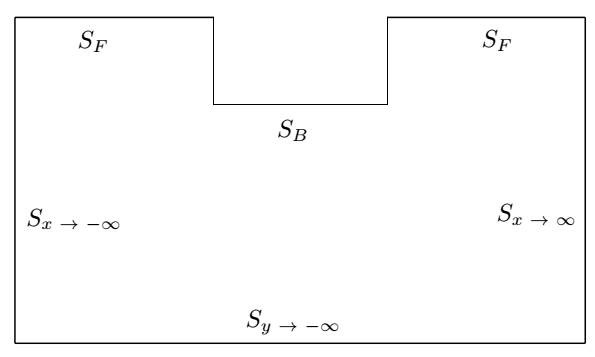
\includegraphics[width=9cm, height=5cm]{illustration.png} 
	\caption{Illustration of the fluid domain and the boundaries in 2D, where $S_F$ is the free surface and $S_B$ is the rigid body boundary.}
\label{illustration}
\end{figure}

\subsection{The boundary value problem for the Green function in 2D}
The 2D wave Green function where $g(x,y,t) = Re \big\{ G(x,y) e^{i \omega t} \big\}$ and $K = \frac{\omega^2}{g}$ is:
\begin{align} \label{G}
G = log(\frac{r}{r_1}) + Re\{f_1\} + i Re\{f_2\}
\end{align}
where:
\begin{align*}
r &= \sqrt{(x-\xbar)^2+(y-\ybar)^2}\\[0.5 em]
r_1 &= \sqrt{(x-\xbar)^2+(y+\ybar)^2}\\[0.5 em]
f_1 = 2 PV \int_0^\infty \frac{e^{-i k (z - \overline{\zeta}^*)}}{K - k} dk &= -2 e^Z (E_1(Z) + log(Z) - log(-Z)) \hspace{2mm} \rightarrow \hspace{2mm} \pm 2 \pi i e^Z \text{  as  } x-\xbar \hspace{2mm} \rightarrow \hspace{2mm} \pm \infty \\[0.5 em]
f_2 &= 2 \pi i e^Z 
\end{align*}

where $z = x + iy$ and $\overline{\zeta}^* = \xbar - i \ybar$ and $Z = K(y + \ybar) - i K (x - \xbar)$ and $E_1$ is the exponential integral. \\

The boundary value problem for the green function G is:
\begin{align}
& \nabla^2 G = 0 \quad && \text{in the fluid domain}\\[0.5 em]
& \frac{\dd G}{\dd y} = K G \quad && \text{at the free surface where $y=0$}\\[0.5 em]
& \phi_2 \frac{\dd G}{\dd n} - G \frac{\dd \phi_2}{\dd n} = 0  \quad && \text{at the free surface where $y=0$ and on } S_\infty \text{ and } S_{- \infty} \\[0.5 em]
& \frac{\dd G}{\dd (\pm x)} = -i K G \quad && \text{on } S_\infty \text{ and } S_{- \infty}\\[0.5 em]
& \rvert \nabla G \rvert \rightarrow 0 \quad && \text{as y} \rightarrow - \infty
\end{align}

Using Green's theorem, we find an integral equation for the heave problem with a free surface as follows:
\begin{equation} \label{int.eq.}
	\int_{S_B + S_F + S_\infty + S_{-\infty}}(\phi_2 \frac{\dd G}{\dd n} - G \frac{\dd \phi_2}{\dd n})dS = \begin{cases}
		0, & \text{$\vec{\xbar}$ outside the fluid domain}.\\
		\pi \phi_2(\vec{\xbar}), & \text{$\vec{\xbar}$ on the boundary}.\\
    	2\pi \phi_2(\vec{\xbar}), & \text{$\vec{\xbar}$ inside the fluid domain}.
	\end{cases} 
\end{equation}
As presented in the BVP for the heave potential $\phi_2$ and the Green function $G$, we have that:
$$\frac{\dd \phi_2}{\dd y} = K \phi_2 \quad \text{and} \quad \frac{\dd G}{\dd y} = KG$$ on the free surface $S_F$
which means that the integral in (\ref{int.eq.}) becomes zero at the free surface.\\[1 em]

We also get zero for the integral over the boundaries $S_\infty$ and $S_{- \infty}$, since we have that: 
$$\frac{\dd \phi_2}{\dd (\pm x)} = -i K \phi_2 \quad \text{and} \quad \frac{\dd G}{\dd (\pm x)} = -i K G$$

On the bottom where $y \hspace{1mm} \rightarrow \hspace{1mm} -\infty$, both functions go towards zero, and therefore the integral there will also be equal to zero.\\[1 em]

So the integral equation (\ref{int.eq.}) for the heave problem with a free surface, when $(\xbar, \ybar)$ is on the body surface $S_B$ becomes:
\begin{equation} \label{int.eq.on_SB}
	\int_{S_B}(\phi_2 \frac{\dd G}{\dd n} - G n_2)dS = \pi \phi_2(\xbar, \ybar)
\end{equation}
and when $(\xbar, \ybar)$ is in the fluid, we get:
\begin{equation}\label{int.eq.in_V}
	\int_{S_B}(\phi_2 \frac{\dd G}{\dd n} - G n_2)dS = 2 \pi \phi_2(\xbar, \ybar)
\end{equation}

\subsection{Numerical solution of the integral equation}
\subsubsection{Discretization of the wetted surface $S_B$}
In order to obtain a numerical solution for the equation, we need to discretize both the equation and the wetted part of the rectangular geometry of width L and draught D. We start by discretization of the geometry, which is done by dividing the three sides of the geometry into N amount of segments, giving us a small increment step in both x and y direction, $dx$ and $dy$. Then we will start at the highest point in the left side of the rectangular geometry, where x point is fixed, then we go downwards in the y direction and make a new point for every $-dy$ step, when we reach the last step which is decided by the number $N$ of the segments, we hold y fixed, while moving in the positive x direction and making a new point for every $dx$ step. The right side of the geometry is also discretized following the same procedure, but this time we will move in the positive y direction, making a new pint after each $dy$ step. Also $S_B = \sum_{m=1}^N S_m$, where each segment $S_m$ is defined by a start coordinate $(x_m^-, y_m^-)$ and a end coordinate $(x_m^+, y_m^+)$. Following plots illustrates this discretization.

\begin{figure}[!htb]
\minipage{0.32\textwidth}
  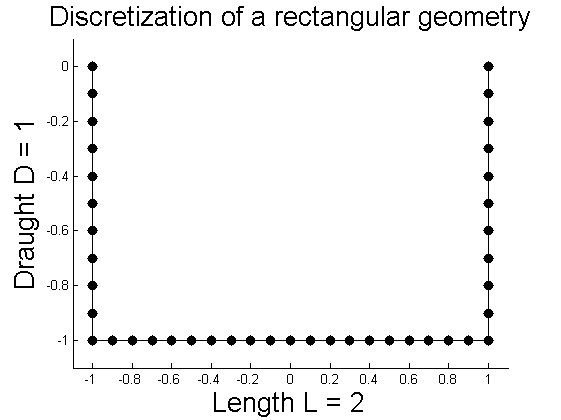
\includegraphics[width=\linewidth]{LD=2.png}
  \caption{N side=10, N bottom=10}\label{LD2}
\endminipage\hfill
\minipage{0.32\textwidth}
  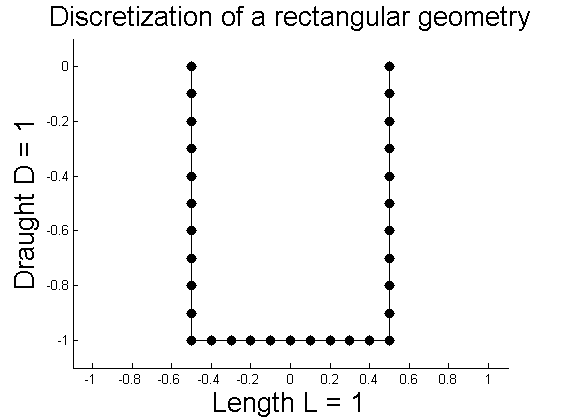
\includegraphics[width=\linewidth]{LD=1.png}
  \caption{N side=10, N bottom=10}\label{LD1}
\endminipage\hfill
\minipage{0.32\textwidth}%
  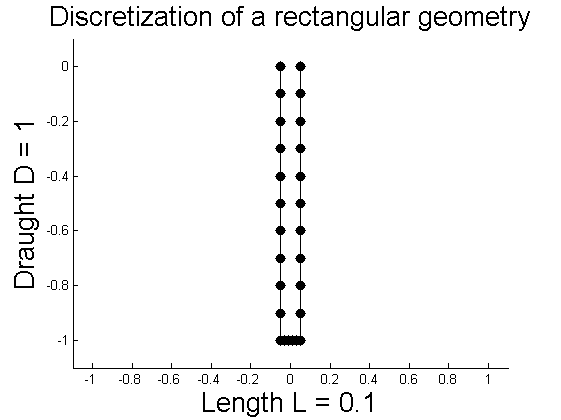
\includegraphics[width=\linewidth]{LD=01.png}
  \caption{N side=10, N bottom=5}\label{LD0.1}
\endminipage
\end{figure}

\subsubsection{Discretization of the integral equation}
Next we need to formulate a discrete version of (\ref{int.eq.on_SB}). A variant of this equation for the incoming wave potential $\phi_0 = (\frac{ig}{\omega})\varphi_0$, is:
\begin{equation}\label{int.eq.on_SB_ver2}
	\int_{S_B}(\varphi_0 \frac{\dd G}{\dd n} - G \frac{\dd \varphi_0}{\dd n})dS = -\pi \varphi_0 \quad \Rightarrow \quad 
	\pi \varphi_0 + \int_{S_B} \varphi_0 \frac{\dd G}{\dd n} dS = \int_{S_B} G \frac{\dd \varphi_0}{\dd n} dS
\end{equation}
where $\varphi_0 = e^{K y - i K x}$, $\frac{\dd \varphi_0}{\dd n} = K(n_2 - i n_1)\varphi_0$ and $K = \frac{\omega^2}{g}$ and G is stated as in (\ref{G}). Since all terms in this equation are given, we can use (\ref{int.eq.on_SB_ver2}) for the purpose of verification of the script we use to solve this equation.\\[1 em]
Discretization of equation (\ref{int.eq.on_SB_ver2}) gives:
\begin{align} \label{disc.eq.}
\pi \varphi_0(\xbar_n, \ybar_n) + \sum_{m=1}^N \varphi_0(\xbar_m, \ybar_m) \int_{S_m} \frac{\dd G}{\dd n}dS = \sum_{m=1}^N \frac{\dd \varphi_0}{\dd n} \bigg\vert_{(\xbar_m, \ybar_m)} \int_{S_m} G dS
\end{align}
For the left hand side of equation (\ref{disc.eq.}),the log term contributions of Green function $G$ are obtained by:
\begin{align} \label{LHS-log}
& \int_{S_m}\frac{\dd}{\dd n}(log r + log r_1)dS \nonumber \\
& = -Im\bigg(log[x + iy - \xbar_n - i\ybar_n]\bigg\vert_{x_m^- + i y_m^-}^{x_m^+ + i y_m^+}\bigg)-Im\bigg(x + iy - \xbar_n + i\ybar_n]\bigg\vert_{x_m^- + i y_m^-}^{x_m^+ + i y_m^+}\bigg)
\end{align}
For the other part of $G$ on the left hand side of (\ref{disc.eq.}), we can use the midpoint rule to get the following integral:
\begin{align} \label{LHS-wp}
& \int_{S_m} \frac{\dd}{\dd n}(Re \{ f_1 \} + i Re \{ f_2 \}) \nonumber \\
& \simeq \Delta S_m \bigg( n_1 K [Im(f_1) + i Im(f_2)] + n_2 K [Re(f_1) + i Re(f_2)] \bigg) \bigg\vert_{(\xbar_m, \ybar_m)}
\end{align}
where $\Delta S_m$ is the length of segment $S_m$.\\[1 em]
Discretization of the right hand side of (\ref{disc.eq.}) gives:
\begin{align} \label{RHS}
\sum_{m=1}^N \frac{\dd \varphi_0}{\dd n} \bigg\vert_{(\xbar_m, \ybar_m)} \int_{S_m} (log r + log r_1 + Re \{ f_1 \} + i Re \{ f_2 \} ) dS
\end{align}
where the log terms are integrated using 2-point Gaussian quadrature rule, while the other terms is integrated by the midpoint rule.\\[1 em]

To be able to estimate the preceding discrete equations, we first need to discretize the geometry we want to consider as described in the previous section, then we give these discretized coordinate information to a numerical program that calculates the normal vectors, estimates points for Gaussian integration and also midpoints for use in the midpointrule for integration and then carries out the integration to obtain the solution.\\[1 em]

For the unit normal vector $\textbf{n} = (n_1 , n_2)$ which is the normal vector on segment $S_m$, pointing out of the fluid, we have the following expressions:\\
$$n_1 = -\frac{dy}{dS} \quad , \quad n_2 = \frac{dx}{dS} \quad \text{where} \quad dS = \sqrt{(dx)^2 + (dy)^2} $$ 

The evaluation points for the 2-points Gaussian integration are given by:
\begin{align*}
& x_m^{(1,2)} = \pm \frac{1}{2} (x_m - x_{m-1}) \frac{\sqrt{3}}{3} + \frac{1}{2} (x_{m-1} + x_m)
& y_m^{(1,2)} = \pm \frac{1}{2} (y_m - y_{m-1}) \frac{\sqrt{3}}{3} + \frac{1}{2} (y_{m-1} + y_m)
\end{align*}

since both the RHS and the LHS of (\ref{disc.eq.}) have an imaginary and a real part, we can check if we get equality between both sides, by checking that real part of the RHS is equal to the real part of the LHS, and the imaginary part of the RHS is equal to the imaginary part of the LHS.\\[1 em]

The numerical results in figures (\ref{L2_KD1.2}) and (\ref{L2_KD0.9}), compares the real and imaginary part of the right and left hand side of (\ref{disc.eq.}) for a rectangular geometry with length $L=2$ and draught $D=1$ and $K D = \frac{\omega^2}{g} D = 1.2$ and $0.9$. \\[1 em]

\begin{figure}[H]
\minipage{0.51\textwidth}
  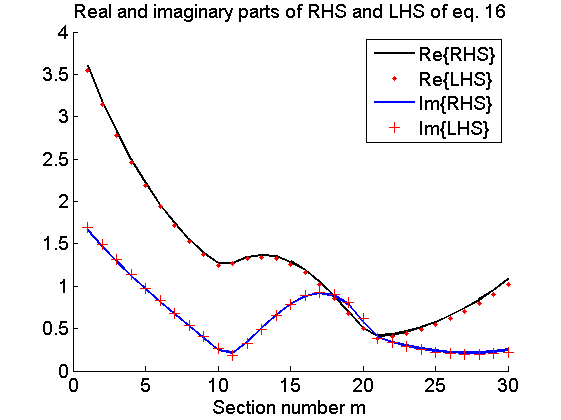
\includegraphics[width=\linewidth]{L2_KD=12.png}
  \caption{$L = 2 , \quad D = 1 , \quad K D = 1.2$}\label{L2_KD1.2}
\endminipage\hfill
\minipage{0.51\textwidth}
  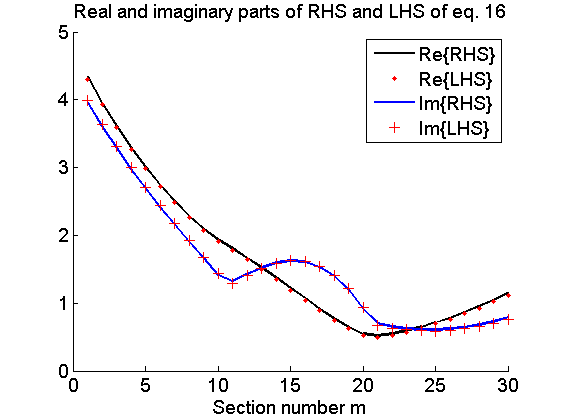
\includegraphics[width=\linewidth]{L2_KD=09.png}
  \caption{$L = 2 , \quad D = 1 , \quad K D = 0.9$}\label{L2_KD0.9}
\endminipage
\end{figure}

As we can see, there is perfect equality of the right and left hand side of (\ref{disc.eq.}), solved numerically, which means the program works properly and we can proceed to finding a solution for the heave problem. But first we need to make some modifications to the script we are using.\\[1 em]

\subsection{Heave potential $\phi_2$}
The integral equation to be solved is:
\begin{align} \label{phi2_eq}
& -\pi \phi_2(\xbar, \ybar) + \int_{S_B} \phi_2 \frac{\dd G}{\dd n} dS = \int_{S_B} G n_2 dS
\quad \Rightarrow \quad -\pi \phi_{2,n} + \sum_{m=1}^N \phi_{2,m}\int_{S_B} \frac{\dd G}{\dd n} dS = \int_{S_B} G n_2 dS
\end{align} 

Where $\frac{\dd G}{\dd n}$ is solved numerically by implementing (\ref{LHS-log}) and (\ref{LHS-wp}), as before, while we modify the term $\frac{\dd \phi}{\dd n}$ to $n_2$ so the RHS is evaluated by summing up all the three parts of $G$ and then multiply it with the normal vector $n_2$. We also need to change the sign in the first term in the parenthesis on the LHS of (\ref{phi2_eq}) to $-\pi$, which differs from the test case. $\phi_2$ is then easily estimated by solving the linear system $A \phi_2 = B$, where $A$ is the part in the parenthesis and B is the RHS of (\ref{phi2_eq}). Following this numerical procedure, we can evaluate an array $\phi_2$ that is a numerical representation of the heave potential $\phi_2$ at the midpoint of each segment $S_m$ of the rigid body surface $S_B$.

\begin{figure}[H]
\minipage{0.51\textwidth}
  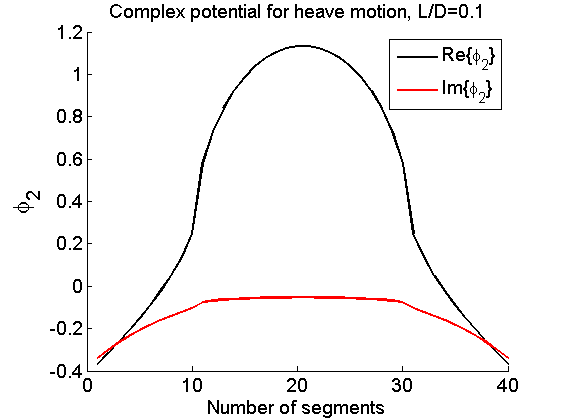
\includegraphics[width=\linewidth]{phi2_box1_12.png}
  \caption{$L = 2 , \quad D = 1 , \quad K D = 1.2$}\label{box1_1.2}
\endminipage\hfill
\minipage{0.51\textwidth}
  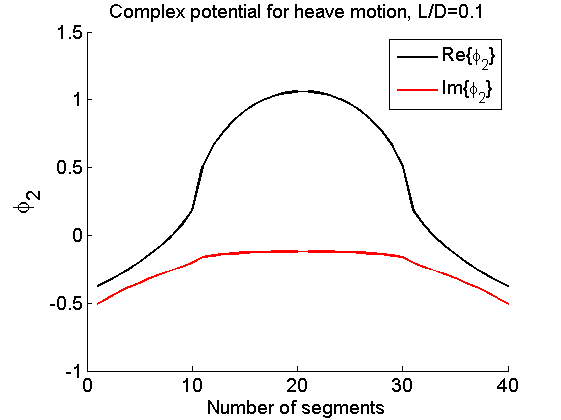
\includegraphics[width=\linewidth]{phi2_box1_09.png}
  \caption{$L = 2 , \quad D = 1 , \quad K D = 0.9$}\label{box1_0.9}
\endminipage
\end{figure}

\begin{figure}[H]
\minipage{0.51\textwidth}
  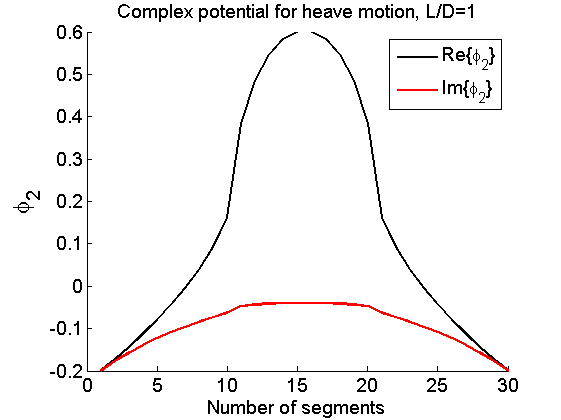
\includegraphics[width=\linewidth]{phi2_box2_12.png}
  \caption{$L = 1 , \quad D = 1 , \quad K D = 1.2$}\label{box2_1.2}
\endminipage\hfill
\minipage{0.51\textwidth}
  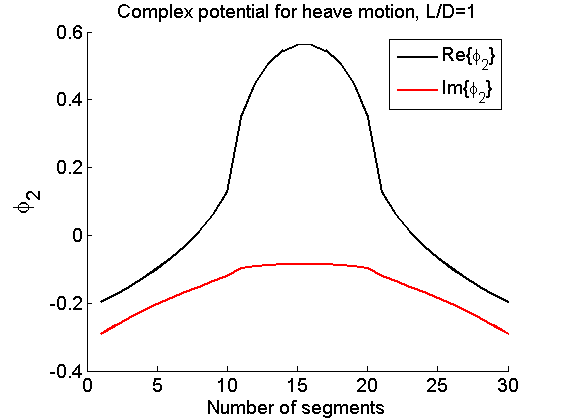
\includegraphics[width=\linewidth]{phi2_box2_09.png}
  \caption{$L = 1 , \quad D = 1, \quad K D = 0.9$}\label{box2_0.9}
\endminipage
\end{figure}

\begin{figure}[H]
\minipage{0.51\textwidth}
  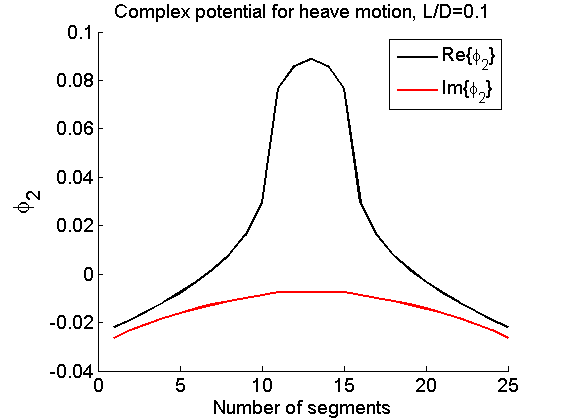
\includegraphics[width=\linewidth]{phi2_box3_12.png}
  \caption{$L = 0.1 , \quad D = 1 , \quad K D = 1.2$}\label{box3_1.2}
\endminipage\hfill
\minipage{0.51\textwidth}
  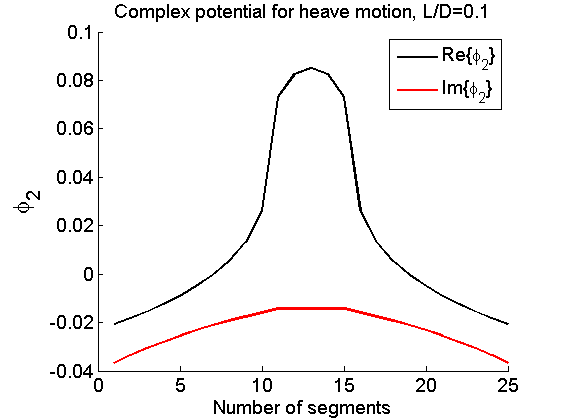
\includegraphics[width=\linewidth]{phi2_box3_09.png}
  \caption{$L = 0.1 , \quad D = 1 , \quad K D = 0.9$}\label{box3_0.9}
\endminipage
\end{figure}

\subsection{Far field behaviour of $\phi_2$}
The potential has the following far field behaviour:
\begin{align}
\phi_2 (\xbar, \ybar) \quad &\rightarrow \quad A_2^{-\infty} e^{K \ybar + i K \xbar} ,  \hspace*{0.5cm} \xbar \rightarrow - \infty \\
\phi_2 (\xbar, \ybar) \quad &\rightarrow \quad A_2^{\infty} e^{K \ybar - i K \xbar} ,  \hspace*{0.5cm} \xbar \rightarrow \infty
\end{align}
where $K = \frac{\omega^2}{g}$ and the complex constants $A_2^{\pm \infty}$ are obtained as integrals over the wetted body surface, using the following integral equation that yields for an evaluation point $(\xbar, \ybar)$ in the fluid:
\begin{align}
2 \pi \phi_2(\xbar, \ybar) = \int_{S_B} \Big(\phi_2 \frac{\dd G}{\dd n} - G \frac{\dd \phi_2}{\dd n}\Big) dS
\end{align}
(21)-(23) give us the following integral for the complex constants $A_2^{\pm \infty}$:
\begin{align}
A_2^{\pm \infty} &= \frac{1}{2 \pi e^{K \ybar \mp i K \xbar}} \int_{S_B} (\phi_2 \frac{\dd G}{\dd n} - G \frac{\dd \phi_2}{\dd n}) dS\\
&=  \frac{1}{2 \pi e^{K \ybar \mp i K \xbar}} \int_{S_B} \bigg(\phi_2(n_1 \frac{\dd}{\dd x} + n_2 \frac{\dd}{\dd y})G - G n_2\bigg) dS\\
&=  \frac{1}{2 \pi e^{K \ybar \mp i K \xbar}} \int_{S_B} \Bigg[ \bigg( \phi_2 (n_1 \frac{\dd}{\dd x} +n_2 \frac{\dd}{\dd y}) - n_2 \bigg) 2 \pi i e^{K(y + \ybar) \mp iK(x-\xbar)} \Bigg]
\end{align}
The calculations above with some simplifications give us the following integrals for the evaluation of $A_2^{\pm \infty}$:

\begin{align}
&A_2^{-\infty} = i \int_{S_B} \big[ \phi_2 \Big( n_1 \frac{\dd \varphi_0 }{\dd x} + n_2 \frac{\dd \varphi_0}{\dd y} \Big) - n_2 \Big] d S, \hspace*{0.5cm} \xbar \rightarrow - \infty\\
&A_2^{-\infty} = i \int_{S_B} \big[ \phi_2 \Big( \frac{\dd \varphi_0}{\dd n} \Big) - n_2 \Big] e^{K y + i K x} d S, \hspace*{0.5cm} \xbar \rightarrow - \infty\\
&A_2^{-\infty} = \int_{S_B} \big[  \phi_2 \Big( K n_2 - i K n_1  \Big) - n_2 \Big] \varphi_0 d S, \hspace*{0.5cm} \xbar \rightarrow - \infty
\end{align}
The exact same calculation for when $\xbar \rightarrow \infty$ give us:
\begin{equation}
A_2^{\infty} = \int_{S_B} \big[  \phi_2 \Big( K n_2 + i K n_1  \Big) - n_2 \Big] \overline{\varphi_0} d S, \hspace*{0.5cm} \xbar \rightarrow \infty
\end{equation}

where $\overline{\varphi_0} = conj({\varphi_0}) = e^{K y + i K x}$ and we have used $\frac{\dd \varphi_0}{\dd n} = K(n_2 - i n_1) \varphi_0$.

\subsection{Added mass and damping}
We can now find the force associated with the heave mode of motion by using the following expression:
\begin{equation}
F_2 (t) = - \dot{U}_2 a_{22} - U_2 b_{22} =  Re\{- i\omega^2\ \xi_2 f_{22} e^{i \omega t} \}
\end{equation}

where $f_{22}$ is the force coefficient analogous to the added mass coefficients, but which is complex as a result of the free surface and the real and imaginary parts depend on the frequency $\omega$, So the force coefficient $f_{22}$ takes the form:

\begin{align}
&f_{22} = a_{22} + \frac{b_{22}}{i \omega} = \rho \int_{S_B} \phi_2 n_2 dS\\[1 em]
&\frac{f_{22}}{\rho \omega^2 D^2} = \frac{a_{22}}{D^2 \rho} - i \frac{b_{22}}{\omega \rho D^2}\\[1 em]
\Rightarrow \quad &\frac{a_{22}}{\rho D^2} = Re\{f_{22}\} \quad , \quad \frac{b_{22}}{\rho \omega D^2} = -Im\{f_{22}\}
\end{align}

By using the numerical solution of $\phi_2$ along the wetted body surface $S_B$, we can calculate the added mass $a_{22}$ and damping $b_{22}$ for the wavenumber range $0 < KD=\frac{\omega^2 D}{g} < 2$ for the three geometries:

\begin{figure}[H]
\minipage{0.33\textwidth}
  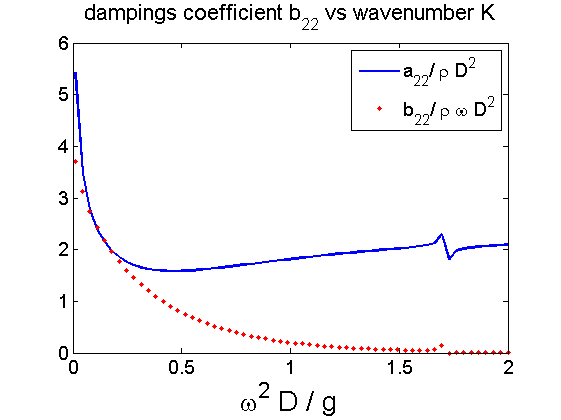
\includegraphics[width=\linewidth]{ad_mass_box1.png}
  \caption{$a_{22}$ and $b_{22}$ of the\\ rectangular geometry where\\ $\frac{L}{D}=2$}\label{add_mass_box1}
\endminipage
\minipage{0.33\textwidth}
  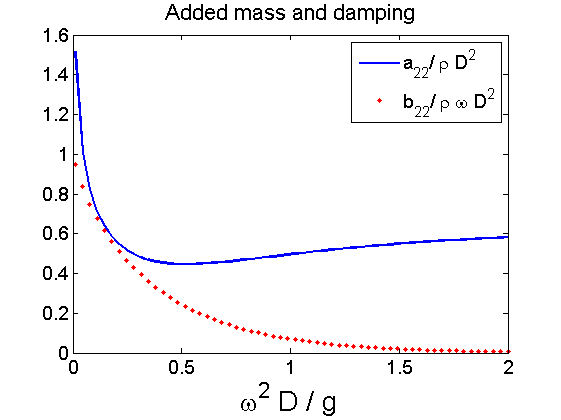
\includegraphics[width=\linewidth]{ad_mass_box2.png}
  \caption{$a_{22}$ and $b_{22}$ of the\\ rectangular geometry where\\ $\frac{L}{D}=1$}\label{add_mass_box2}
\endminipage
\minipage{0.33\textwidth}%
  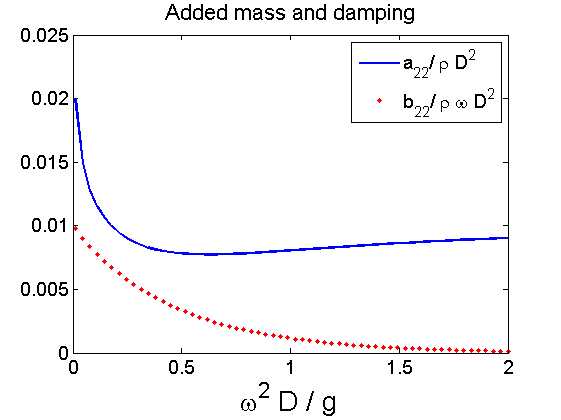
\includegraphics[width=\linewidth]{ad_mass_box3.png}
  \caption{$a_{22}$ and $b_{22}$ of the\\ rectangular geometry where\\ $\frac{L}{D}=0.1$}\label{add_mass_box3}
\endminipage
\end{figure}

As we can see from the figures (\ref{add_mass_box1})-(\ref{add_mass_box3}), $\frac{b_{22}}{\rho \omega D^2} \rightarrow 4$, while $\frac{a_{22}}{\rho D^2}$ tends to infinity, in the long wavelength limit as $\frac{\omega^2 D}{g} \rightarrow 0$, but they both tend to zero as the wavenumber goes toward $2$. We can also see that for a geometry where $L/D = 2$, the numerical solution oscillates a bit around $\frac{\omega^2 D}{g} \approx 1.7$, but I'm not able to explain this behaviour.\\[1em]

We can also calculate $b_{22}$ from the energy balance. The time averaged work done by the force on the body is given by:
\begin{align}
\overline{W} &= F_2 \cdot U_2 = \overline{\dot U_2 U_2}a_{22} + U_2^2 b_{22}\\
&= \overline{E}^{\hspace{1mm} +} c_g + \overline{E}^{\hspace{1mm} -} c_g\\
&= \frac{1}{2} \vert \xi_2 \vert^2 \omega^2 b_{22}\\
&= \frac{1}{2} \rho g c_g \big(\vert amp_2^{+ \infty} \vert^2 + \vert amp_2^{- \infty} \vert^2\big)\\
\Rightarrow b_{22} &= \frac{\overline{W}}{\frac{1}{2} \vert \xi_2 \vert^2 \omega^2} = \frac{\rho g \Big( \big\vert \frac{amp_2^{+ \infty}}{\xi_2} \big\vert^2 +  \big\vert \frac{amp_2^{- \infty}}{\xi_2} \big\vert^2 \Big) \frac{g}{2 \omega}}{\omega^2} \label{work}
\end{align}

where we have used that $c_g = \frac{1}{2}c_f = \frac{1}{2} \frac{\omega}{k} = \frac{1}{2} \frac{\omega}{\omega^2 / g} = \frac{g}{2 \omega}$, and the amplitudes are given by:
$${amp}_2^{- \infty} = \xi_2 A_2^{-\infty} \omega^2 / g $$
$${amp}_2^{+ \infty} = \xi_2 A_2^{\infty} \omega^2 / g $$

Substituting these in (\ref{work}) gives:
\begin{align}
\frac{b_{22}}{\rho \omega} &= \frac{g^2}{2 \omega^4} \Bigg( \bigg\vert \frac{\xi_2 A_2^{+\infty} \frac{\omega^2}{g}}{\xi_2} \bigg\vert^2 + \frac{\xi_2 A_2^{-\infty} \frac{\omega^2}{g}}{\xi_2} \bigg\vert^2 \Bigg)\\
&= \frac{g^2}{2 \omega^4} \bigg( \big\vert A_2^{+ \infty} \big\vert^2 + \big\vert A_2^{- \infty} \big\vert^2 \bigg) \frac{\omega^4}{g^2}\\
&= \frac{1}{2} \Big( \big\vert A_2^{+ \infty} \big\vert^2 + \big\vert A_2^{- \infty} \big\vert^2 \Big) \label{b22_2}
\end{align}

As shown above we can calculate $b_{22}$ using the energy method, also by the expression in (\ref{b22_2}). We can see a visualization of these results together with the results obtained by direct calculation and also by using the Froude-Krylov approximation in figures (\ref{add_mass_box1_2})-(\ref{add_mass_box3_2}) .


\subsection{Comparison of the approximate solution to the full calculation of the damping force $b_{22}$}
For a freely floating, vertical spar buoy(small water plane area and large mass) in 2D, with draught D and length L, we can compute an approximate solution for the exciting force, using the Froude-Krylov approximation as follows:

\begin{align}
X_2^{FK} &\approx -i \omega \rho \int_{S_B} \phi_0 n_2 dS = -i \omega \rho \int_{S_B} \frac{i g}{\omega} \varphi_0 n_2 dS \nonumber\\[0.5 em]
&= \rho g \int_{S_B} \varphi_0 n_2 dS = \rho g \int_{S_B} e^{Ky - iKx}  \frac{dx}{dS} dS \nonumber\\[0.5 em]
&= \rho g \int_{-L/2}^{L/2} e^{-KD - iKx} dx = 2 \rho g e^{-KD}\frac{\sin(KL/2)}{K}\nonumber\\
&=\rho g L e^{-KD} \frac{\sin(KL/2)}{KL/2} \label{FK}
\end{align}
For a narrow geometry which has a small length compared to the wave-length, where the long-wave approximation ($KL<<1$) yields, we have:
\begin{equation}
\sin\Big(\frac{KL}{2}\Big) \approx \frac{KL}{2} \quad \Rightarrow \quad X_2 = \rho g L e^{-KD}
\end{equation}

In this representation for the exciting force, we assume that the pressure field is not affected by the presence of the body, and the exciting force can be determined from the incident wave potential by itself. Once we have the exciting force $X_2$, we can use it to find the damping force.

\begin{equation}
b_{22} = \frac{\vert X_2 \vert^2}{2 \rho g c_g} = \frac{\big\vert \rho g L e^{-KD} \big\vert^2}{\rho g^2 / \omega} = \omega \rho L^2 e^{-2 KD}
\end{equation}
where we have used that $c_g = \frac{g}{2 \omega}$.\\[1 em]

\begin{figure}[H]
\minipage{0.33\textwidth}
  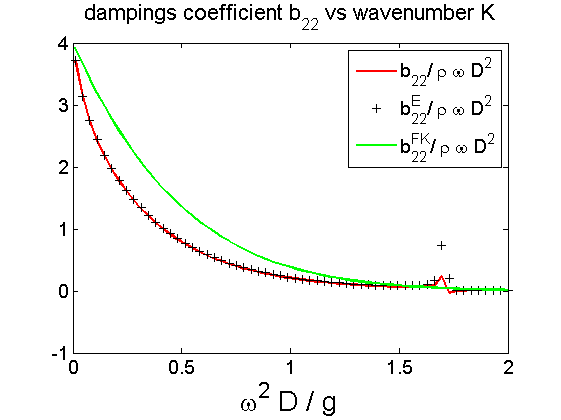
\includegraphics[width=\linewidth]{ad_mass_box1_2.png}
  \caption{}\label{add_mass_box1_2}
\endminipage
\minipage{0.33\textwidth}
  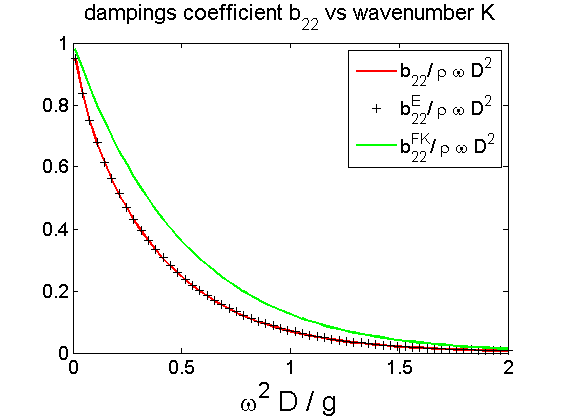
\includegraphics[width=\linewidth]{ad_mass_box2_2.png}
  \caption{}\label{add_mass_box2_2}
\endminipage
\minipage{0.33\textwidth}%
  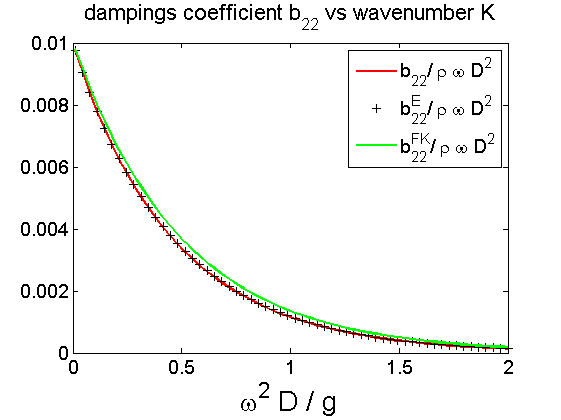
\includegraphics[width=\linewidth]{ad_mass_box3_2.png}
  \caption{}\label{add_mass_box3_2}
\endminipage
\end{figure}

In the figures above, we compare the damping-coefficients $b_{22}$ that we obtain using three different methods for the three rectangular geometries. The red grapth is the results obtained by using the numerical solution of $\phi_2$, while the black graph shows $b_{22}$ obtained from the energy balance and the green graph shows the damping obtained by using the Froude-Krylov approximation.\\
As we can see the results from direct integration and using energy balance are exactly the same, while Froude-Krylov give a bit higher values, but is still a good approximation that gets more accurate az the box gets thinner. All graphs start at $L^2$ for $K=0$, and they all go towards zero as $k \rightarrow 2$.


\section{The diffraction problem}
In the diffraction problem the geometry is held fixed. The interaction of the incoming wave field with the geometry results in a field of scattered waves. The diffraction potential is represented by:

\begin{equation}
\Phi_D(x,y,t) = Re \Big( A (\phi_0(x,y) + \phi_7(x,y) ) e^{i \omega t} \Big) = \Phi_D(x,y,t) = Re \Big( A \phi_D(x,y) e^{i \omega t} \Big) 
\end{equation}
where: 

A is the amplitude of the incoming waves\\
$\phi_0(x,y) = \big(\frac{ig}{\omega}\big) \varphi_0 = \big(\frac{ig}{\omega}\big) e^{K y - iKx}$, is the incoming wave potential in the case of deep water.\\
and $\phi_7$ is the unknown scattering potential.\\[1 em]

\begin{align}
&\nabla^2 \phi_7 = 0  \quad  \quad && \text{in the fluid}\\
&\frac{\dd \phi_D}{\dd n} = \frac{\dd \phi_0}{\dd n} + \frac{\dd \phi_7}{\dd n}= 0 \quad \Rightarrow \quad \frac{\dd \phi_0}{\dd n} = - \frac{\dd \phi_7}{\dd n} \quad  \quad && \text{on } S_B\\
&-\frac{\omega^2}{g} \phi_7 + \frac{\dd \phi_7}{\dd y} = 0 \quad \Rightarrow \quad \frac{\dd \phi_7}{\dd y} =  K \phi_7 \quad  \quad &&\text{at the free surface } S_F \text{ where } y=0\\
& \frac{\dd \phi_7}{\dd (\pm x)} = \mp i \phi_7 \quad  \quad && \text{ at } S_{\pm \infty}\\
& \vert \nabla \phi_7 \vert \rightarrow 0 \quad  \quad && y \rightarrow - \infty
\end{align} 

The integral equation to determine the sum $\phi_D = \phi_0 + \phi_7$ for a point $(\xbar, \ybar)$ on $S_B$ is:
\begin{align} \label{diff_pot}
- \pi \phi_D(\xbar, \ybar) + \int_{S_B} \phi_D \frac{\dd G}{\dd n}dS = -2 \pi \phi_0(\xbar, \ybar)
\end{align}

The scattering potential $\phi_7$ can be considered as the disturbance associated with a forced normal velocity on the body surface equal and opposite to that of the incident wave
By solving the integral equation (\ref{diff_pot}), we get the following results for the diffraction potential $\phi_D$ for the three rectangular geometries discretized as in figures (\ref{LD2})-(\ref{LD0.1}).

\begin{figure}[H]
\minipage{0.33\textwidth}
  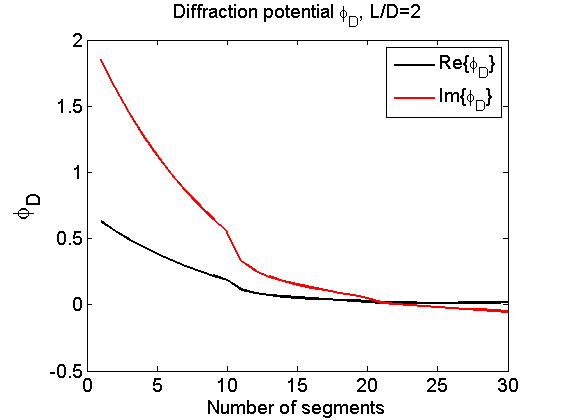
\includegraphics[width=\linewidth]{diff_box1.png}
  \caption{}\label{diff_box1}
\endminipage
\minipage{0.33\textwidth}
  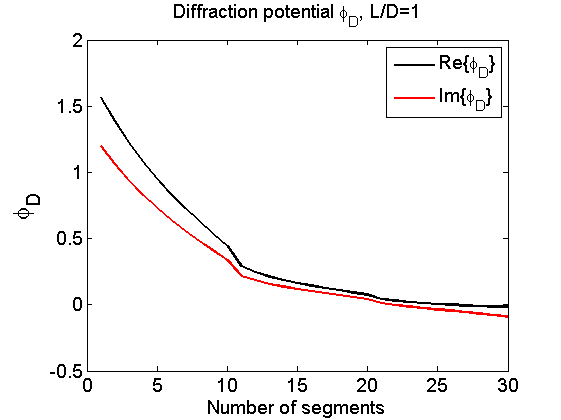
\includegraphics[width=\linewidth]{diff_box2.png}
  \caption{}\label{diff_box2}
\endminipage
\minipage{0.33\textwidth}%
  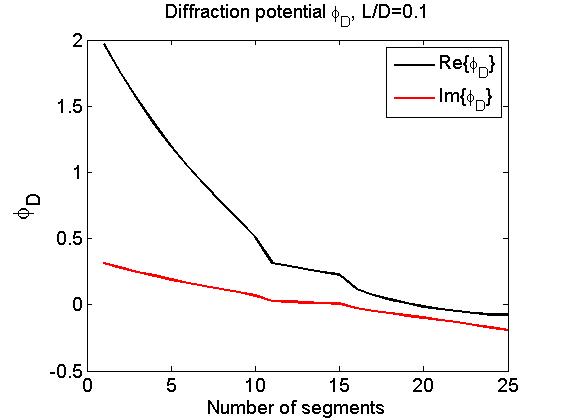
\includegraphics[width=\linewidth]{diff_box3.png}
  \caption{}\label{diff_box3}
\endminipage
\end{figure}

\subsection{The exciting force}
by solving the integral equation (\ref{diff_pot}) numerically, we can use the results for the diffraction potential $\phi_D$ to obtain a solution for the exciting force $X_2$, using the following expression.

$$\frac{X_2}{\rho g} = - \frac{i \omega}{g} \int_{S_B} \phi_D n_2 dS = \frac{i \omega}{g} \int_{S_B} (\phi_0 + \phi_7) n_2 dS$$

where: $\phi_0 = \frac{i g}{\omega} \varphi_0$

$$ \Rightarrow \frac{\vert X_2 \vert}{\rho g} = \int_{S_B} \phi_D n_2 dS $$


\begin{figure}[H]
\minipage{0.33\textwidth}
  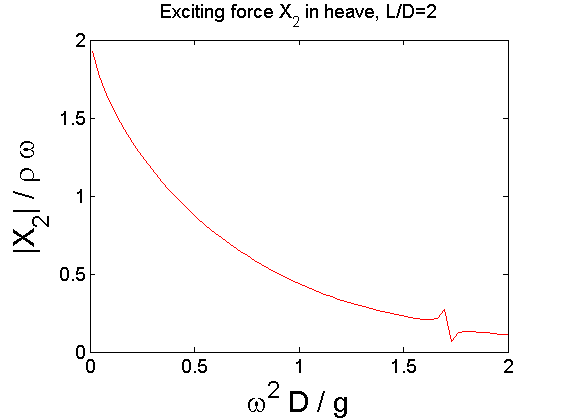
\includegraphics[width=\linewidth]{X2_box1.png}
  \caption{}\label{X2_box1}
\endminipage
\minipage{0.33\textwidth}
  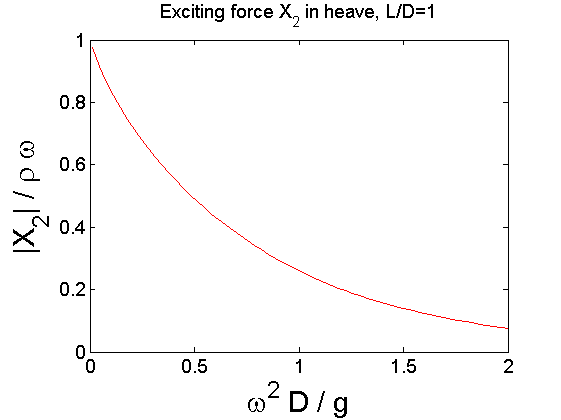
\includegraphics[width=\linewidth]{X2_box2.png}
  \caption{}\label{X2_box2}
\endminipage
\minipage{0.33\textwidth}%
  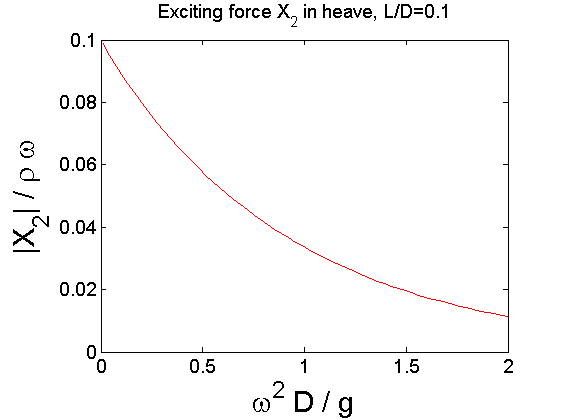
\includegraphics[width=\linewidth]{X2_box3.png}
  \caption{}\label{X2_box3}
\endminipage
\end{figure}

In the figures above we can see plots for the exciting force $\vert X_2 \vert$ in heave by direct integration for the three rectangular geometries.

\subsubsection{Haskind relations}
The exciting force may be obtained by the Haskind relations in several variants, which will provide checks for the numerical computations. These relations are derived as follows:
\begin{align}
\int_{S_B} (\phi_i \frac{\dd \phi_j}{\dd n} - \phi_j \frac{\dd \phi_i}{\dd n}) dS \quad &\Rightarrow \quad \int_{S_B}( \phi_7 \frac{\dd \phi_2}{\dd n} - \phi_2 \frac{\dd \phi_7}{\dd n}) dS = 0 \\
& \Rightarrow \quad \int_{S_B} \phi_7 \frac{\dd \phi_2}{\dd n} dS = \int_{S_B} \phi_2 \frac{\dd \phi_7}{\dd n}
\end{align}
By using condition (48) we get:
\begin{align}
&\int_{S_B} \phi_2 \frac{\dd \phi_7}{\dd n} = \int_{S_B} \phi_2 (- \frac{\dd \phi_0}{\dd n})\\
&\Rightarrow \quad X_2 = - i \omega \rho \int_{S_B} (\phi_0 \frac{\dd \phi_2}{\dd n} - \phi_2 \frac{\dd \phi_0}{\dd n}) dS =  i \omega \rho \int_{S_\infty} (\phi_0 \frac{\dd \phi_2}{\dd n} - \phi_2 \frac{\dd \phi_0}{\dd n}) dS 
\end{align}
Where we have expressed the integral at the geometry by a integral of the control surfaces at $x = \pm \infty$.\\[1 em]

The far field of $\phi_2$ is given by
\begin{equation} \label{int.eq.far}
	\phi_2 = \begin{cases}
		i \omega A_2^\infty e^{Ky - iKx}, & x \rightarrow \infty.\\
		i \omega A_2^{-\infty} e^{Ky + iKx}, & x \rightarrow -\infty.
	\end{cases} 
\end{equation}

\begin{align}
\Rightarrow X_2 &= \rho \int_{S_\infty} (\phi_0 \frac{\dd \phi_2}{\dd n} - \phi_2 \frac{\dd \phi_0}{\dd n}) dS + \rho \int_{S_{-\infty}} (\phi_0 \frac{\dd \phi_2}{\dd n} - \phi_2 \frac{\dd \phi_0}{\dd n}) dS\\
& = \rho \int_{-\infty}^0 (\frac{i g}{\omega} e^{Ky-iKx} (-iK) i \omega A_2^\infty e^{Ky -iKx} - A_2^\infty e^{Ky -iKx}(-iK) i \omega \frac{ig}{\omega} e^{Ky-iKx}) dy\\
& + \rho \int_{-\infty}^0 (\frac{ig}{\omega}e^{Ky-iKx} (-iK) i\omega A_2^{-\infty} e^{Ky+iKx} -A_2^{-\infty} i \omega e^{Ky+iKx} iK \frac{ig}{\omega} e^{Ky-iKx} ) dy\\
& = \rho A_2^{-\infty} 2 ig K \int_{-\infty}^0 e^{2Ky} dy = i \rho g A_2^{- \infty}\\
&\Rightarrow \quad X_2 = \rho \int_{S_\infty} (\phi_0 \frac{\dd \phi_2}{\dd n} - \phi_2 \frac{\dd \phi_0}{\dd n}) dS = i \rho g A_2^{-\infty}\\
& \Rightarrow \frac{X_2^{Haskind, 2}}{\rho g} = i A_2^{- \infty}
\end{align}

we can calculate the exciting force using several other methods, here we will examine four variants.\\[1 em]

\begin{alignat}{3}
&\text{1. Direct integration:} \nonumber \hspace{14 cm}\\
&\frac{\vert X_2 \vert}{\rho g} = \int_{S_B} \phi_D n_2 dS\\[2 em]
&\text{2. First version of the Haskind relation:}\nonumber\\
&\frac{| X_2 |}{i \omega \rho} = -\int_{S_B} (\phi_0 \frac{\dd \phi_2}{\dd n} - \phi_2 \frac{\dd \phi_0}{\dd n}) dS\\
& = - \frac{i g}{\omega} \int_{S_B} (\varphi_0 n_2 - \phi_2 \frac{\dd \varphi_0}{\dd n}) dS\\
& \Rightarrow \frac{|X_2^{HK1}|}{\rho g} = \int_{S_B} (\varphi_0 n_2 - \phi_2 (K(n_2 - in_1)\varphi_0) ) dS\\[2 em]
&\text{3. Second version of the Haskind relation:}\nonumber\\
&\frac{| X_2^{HK2}|}{\rho g} = i A_2^{-\infty}\\[2 em]
&\text{4. Froude-Krylov approximation:}\nonumber\\
&\frac{|X_2|}{\rho g} = L e^{-KD} \frac{sin(KL/2)}{KL/2}
\end{alignat}

The following plots show all four variants for computation of the exciting force as a function of the wavenumber for the three rectangular geometries. As we can see $X_2^{Direct} = X_2^{HK \hspace{1mm} 1, 2}$ and Froude-Krylov method also gives a very good approximation of the exciting force. This means that we can use the Froude-Krylov approximations and also both versions of the Haskind relations to verificate the results we get by direct calculation of the exciting force $X_2$.

\begin{figure}[H]
\minipage{0.33\textwidth}
  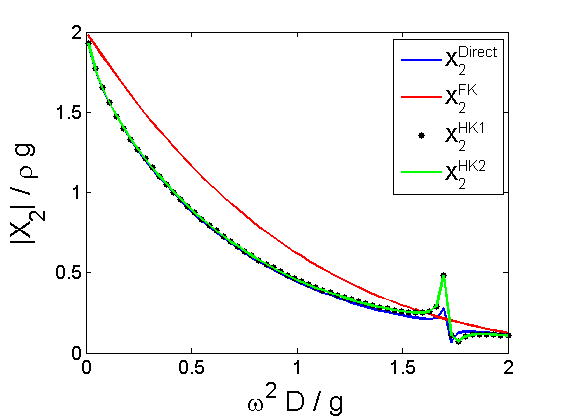
\includegraphics[width=\linewidth]{X2_2_box1.png}
  \caption{}\label{X2_2_box1}
\endminipage
\minipage{0.33\textwidth}
  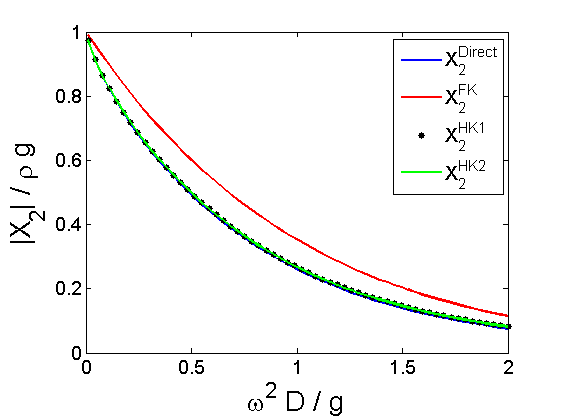
\includegraphics[width=\linewidth]{X2_2_box2.png}
  \caption{}\label{X2_2_box2}
\endminipage
\minipage{0.33\textwidth}%
  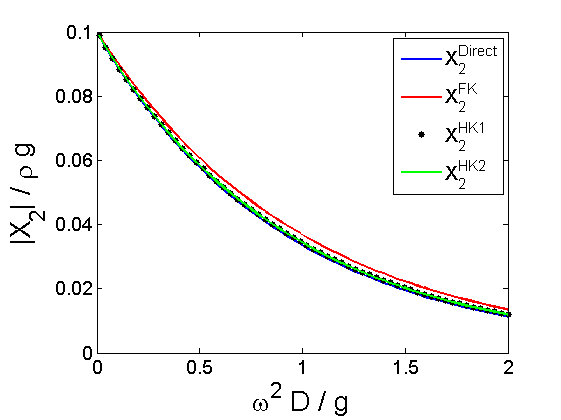
\includegraphics[width=\linewidth]{X2_2_box3.png}
  \caption{}\label{X2_2_box3}
\endminipage
\end{figure}

\section{Body response in heave}

We can use the equation of motion in the heave mode of motion, to obtain an expression for the response$|\xi_2|/A$. We assume that there is no motion in the other modes.\\

The equation of motion reads:
$$Re \Big\{e^{i \omega t} (i \omega)^2 \xi_j M_{ij} \Big\} = Re \Big\{ F_i e^{i \omega t} \Big\}$$
where:
$$F_i = -\xi_j c_{i j} - \xi_j \Big[ (i \omega)^2 a_{i j} + i \omega b_{i j} \Big] + A X_i$$

where $c_{j i}$ are the hydrostatic restoring force coefficients , $b_{i j}$ are the damping coefficients, $a_{i j}$ are the added mass coefficients and $X_i$ is the excitation force. We substitute for $F_i$ and get the following expression:

\begin{align}
&Re \Big\{ e^{i \omega t}\big[(i \omega)^2 \xi_j M_{ij} + \xi_j c_{ij} +\xi_j ((i \omega)^2 a_{ij} + i \omega b_{ij})- AX_i \big]) \Big\} = 0\\
& \Rightarrow \Big[ -\omega^2(M_{ij} + a_{ij})+ i \omega b_{ij} + c_{ij} \Big] \xi_j = AX_i\\
& \Rightarrow \frac{\xi_j}{A} = \frac{X_i}{-\omega^2 (M_{ij} + a_{ij}) + i \omega b_{ij} + c_{ij}}\\
\end{align}

For the heave mode of motion (j=2), we get:
\begin{align}
& \Big[- \omega^2 (M_{2 2} + a_{2 2}) + i \omega b_{2 2} + c_{22} \Big] \xi_2 = A X_{2}\\[1em]
& \Rightarrow \quad \frac{\xi_2}{A} = \frac{X_2}{c_{22} - \omega^2(m + a_{22}) + i \omega b_{22} } 
\label{bodyrespons}
\end{align} 

where $M_{22} = m = \rho \forall$, for a freely floating body and denotes the mass of the geometry which in the case of the freely floating body equals the buoyancy force. $c_{22} = \rho g S$ where $S$ is the water plane area of the geometry that corresponds to the width $L$ of the geometry at the free surface.


\subsection{Resonance frequency}

We get resonance response at the natural frequency where the virtual mass or the inertia forces balances the hydrostatic restoring forces.At or near this frequency, the body will experience a response of large amplitude and a phase shift.\\

\begin{align}
&c_{22} - \omega_n^2 (m + a_{22}) = 0 \quad \Rightarrow \quad \omega_n^2 = \Big( \frac{c_{22}}{a_{22} + m} \Big)\\
& \omega_n^2 = \frac{\rho g L}{\rho D L + a_{22}} = \frac{g}{D}\hspace{1mm}\frac{1}{1 + \frac{a_{22}}{\rho D L}} 
\end{align}

For a rectangular geometry where $L=2D$ and $D=1$, we get the following resonance frequency:
$$\omega_n^2 \frac{D}{g} = \frac{1}{1 + \frac{a_{22}}{2 \rho D^2}} $$

For a geometry where $L=1$ and $D=1$, the resonance frequency is:
$$\omega_n^2 \frac{D}{g} = \frac{1}{1 + \frac{a_{22}}{ \rho D^2}} $$

For the last geometry where $L=0.1$ and $D=1$, we get:
$$ \omega_n^2 \frac{D}{g} = \frac{1}{1 + \frac{a_{22}}{ 0.1 \rho D^2}} $$

We can see from figures (\ref{add_mass_box1}) to (\ref{add_mass_box3}) that the added mass $a_{22}$ does not vary much between $\omega_n^2 \frac{D}{g} = 0.5$ to $1.5$. Also the scaled added masses $\frac{a_{22}}{\rho D^2}$, in this interval are approximately $1.9$, $0.5$ and $0.008$ for boxes with $\frac{L}{D} = 2$, $1$ and $0.1$ respectively. Substituting for these values give us:
$$\frac{L}{D}=2 \quad \Rightarrow \quad \frac{\omega_n^2 D}{g} = 0.51 \quad , \quad 
\frac{L}{D}=1 \quad \Rightarrow \quad \frac{\omega_n^2 D}{g} = 0.67 \quad , \quad 
\frac{L}{D}=0.1 \quad \Rightarrow \quad \frac{\omega_n^2 D}{g} = 0.93 $$

\subsection{Response as a function of frequency}

Following figures show plots for the response amplitude operator $\frac{\xi_2}{A}$ in heave on the three rectangular geometries.

\begin{figure}[H]
 \centering
 
\begin{subfigure}{0.45\textwidth}
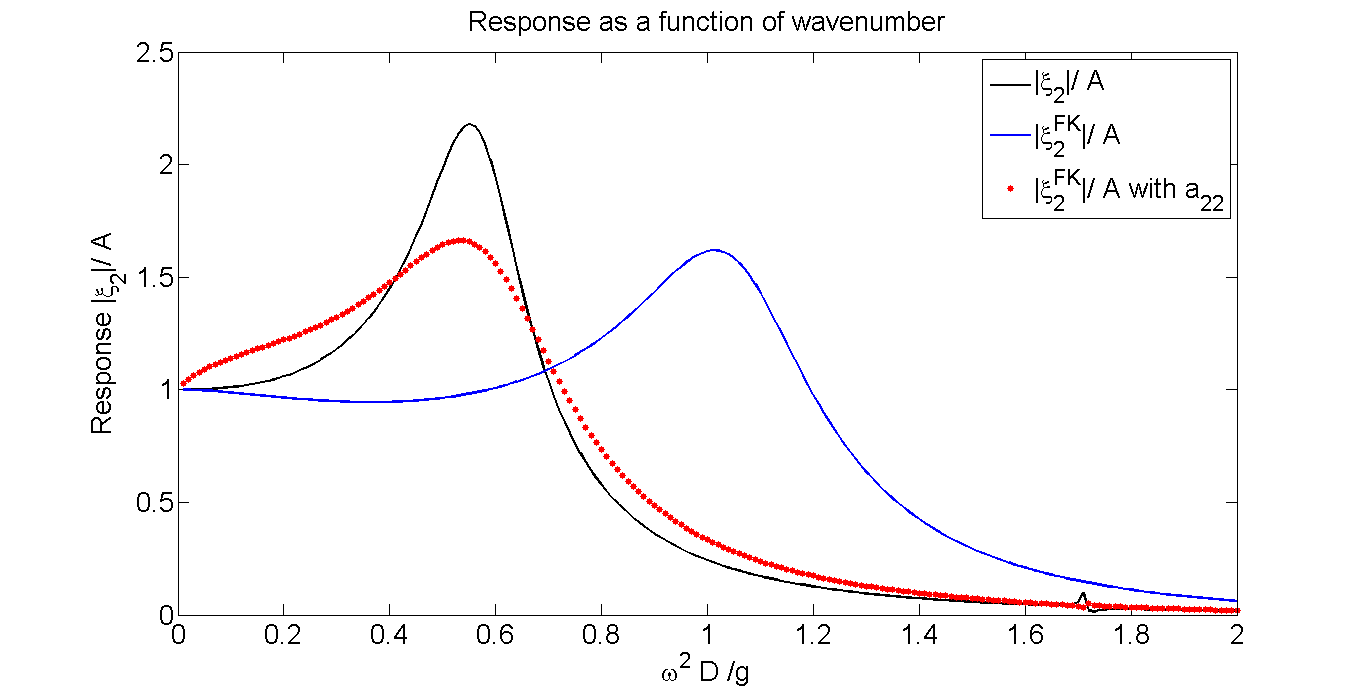
\includegraphics[width=8cm, height=6cm]{respons1.png} 
\caption{}
\label{respons1}
\end{subfigure}
\begin{subfigure}{0.4\textwidth}
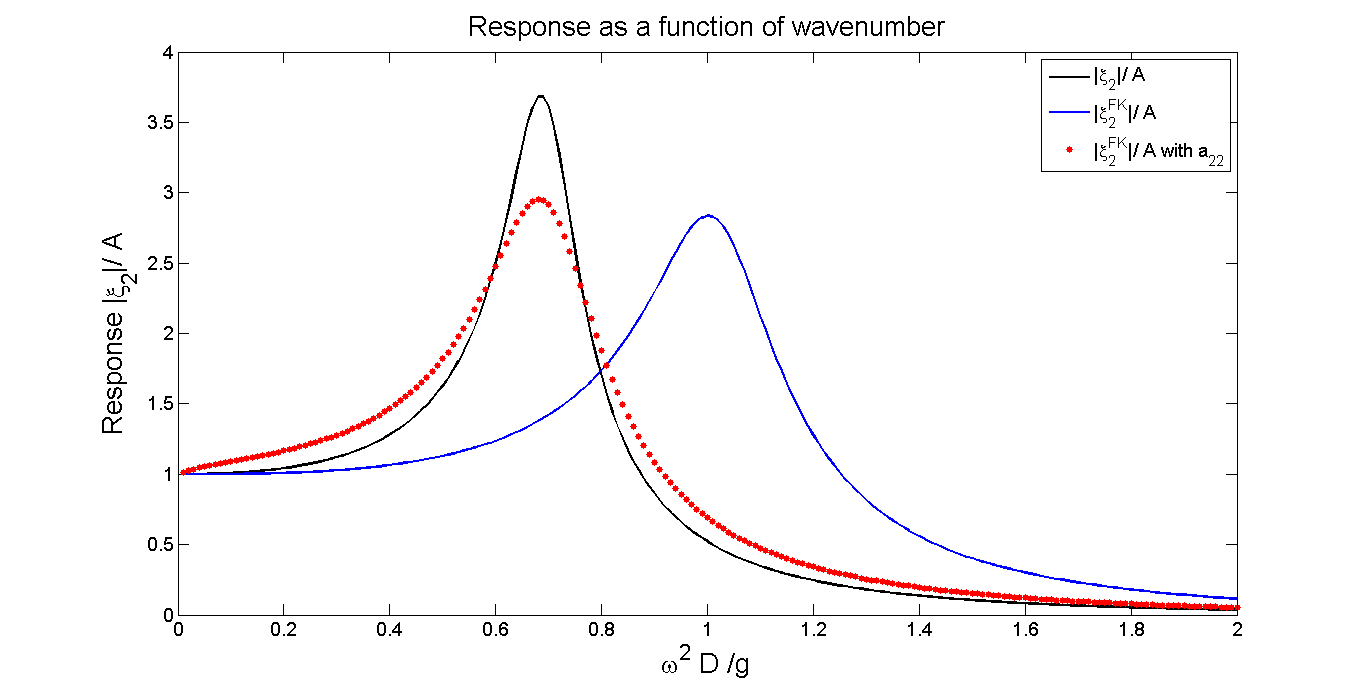
\includegraphics[width=8cm, height=6cm]{respons2.png}
\caption{}
\label{respons2}
\end{subfigure}

\begin{subfigure}{0.6\textwidth}
\centering
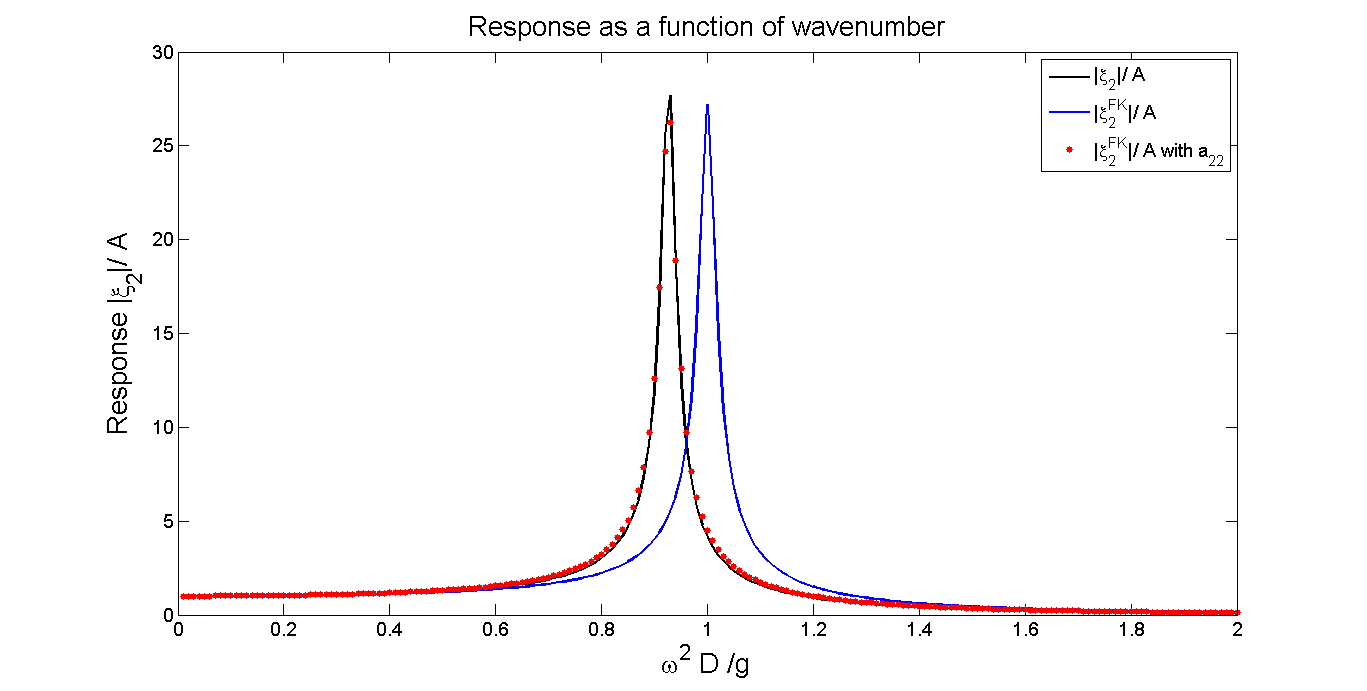
\includegraphics[width=12cm, height=6cm]{respons.png}
\caption{}
\label{respons3}
\end{subfigure}

\caption{}
\label{heave_response}
\end{figure}

As we can see from figure: (\ref{heave_response}), we need the $a_{22}$ to be able to calculate the heave response $\frac{\xi_2}{A}$ correctly.\\[1em]

for a thin box where $\frac{L}{D}=0.1$, at resonance where $\frac{\omega^2 D}{g} = KD \approx 1$ we will get the following response, using the Froude-Krylov approximation:\\
$$\frac{\vert \xi_2^{FK} \vert}{A} = \frac{e^{-KD}}{\vert i L e^{-2KD} \vert} = \frac{2.71}{0.1} = 27.18$$
Which is also shown in figure:(\ref{respons3}).
\newpage
\section{Conclusion}
\begin{enumerate}
\item In the radiation problem, where there are no incoming waves, the wave motion is driven by the oscillatory motion of the geometry. The radiation potentials satisfy the Laplace equation and also the same boundary conditions as the Green function at the free surface and at infinity.\\
The outgoing waves are evaluated by using the far field form of the Green function for an evaluation point inside the fluid.\\

\item To verificate the script we use to evaluate the potential, we can check with a known solution, than proceed to the unknown problem by making some modifications to the code.

\item We can evaluate the far field wave amplitudes, as well as the force and moments such as the added mass and damping, once we have found a solution for the potential.

\item Calculating the damping directly from the potential, gives the same result as using the mean energy flux or energy balance and thus we can use these methods for the purpose of verification of the results. Froude-Krylov approximation gives a bit higher values for bigger boxes, but is still a pretty good approximation, while the calculations give the exact value for a thin box where $\frac{L}{D}=0.1$. The dampings coefficient starts at $L^2$ at $k=0$ and goes towards zero as $k \rightarrow 2$. Several methods to evaluate a quantity is quite useful for checking the validity of the results.

\item The Laplacian scattering potential in the diffraction problem which results from the interaction of the incoming wave field with the geometry, which is held fixed, satisfies the same conditions at the free surface and at infinity as the Green function. This potential is found by solving the diffraction problem where the incoming wave potential in known.

\item The exciting force on the geometry can be obtained by several methods, such as the direct integration of the diffraction potential, using Haskind relation and also by Froude-Krylov approximation. We found out that $X_2^{\text{Direct}} = X_2^{\text{HK 1,2}}$, so they give a check for the results.

\item We need the added mass $a_{22}$ to be able to calculate $\frac{\xi_2}{A}$ correctly, particularly at the resonance frequency.

\end{enumerate}

\newpage
\section{Numerical implementation}
All MATLAB scripts used to obtain the numerical results throughout this report is presented in this section.

\subsection{Geometry discretization}
\begin{verbatim}
% box of draught D and length (width) L, with D as unit length
% left vertical side
D=1;
L=2;
Nside=10;
Nbott=10;
N=Nside+Nbott+Nside;
dy=D/Nside;
dx=L/Nbott;
xp(1)=-L/2;
xm(1)=-L/2;
yp(1)=-dy;
ym(1)=-dy*(1-1);

coord=[xm(1),ym(1),xp(1),yp(1)];

for i=2:Nside;
    xp(i)=-L/2;
    xm(i)=-L/2;
    yp(i)=-dy*i;
    ym(i)=-dy*(i-1);
    coord2=[xm(i),ym(i),xp(i),yp(i)];
    coord=[coord;coord2];
end
for i=1+Nside:Nside+Nbott;
    i1=i-Nside;
    xp(i)=-L/2+dx*i1;
    xm(i)=-L/2+dx*(i1-1);
    yp(i)=-D;
    ym(i)=-D;
    coord2=[xm(i),ym(i),xp(i),yp(i)];
    coord=[coord;coord2];
end
for i=1+Nside+Nbott:Nside+Nbott+Nside;
    i1=i-Nside-Nbott;
    xp(i)=L/2;
    xm(i)=L/2;
    yp(i)=-D+dy*i1;
    ym(i)=-D+dy*(i1-1);
    coord2=[xm(i),ym(i),xp(i),yp(i)];
    coord=[coord;coord2];
end
save -ascii box1.dat coord;
% plot geometry
xa=xm;
xa=[xm,xp(N)];
ya=ym;
ya=[ym,yp(N)];
hold on
axis ([-1.1 1.1 -1.1 0.1])
h1=plot(xa,ya,'k .','MarkerSize',[25])
plot(xa,ya,'k -')
title('Discretization of a rectangular geometry', 'FontSize',20)
xlabel(['Length L = ' num2str(L)],'FontSize',20) % x-axis label
ylabel(['Draught D = ' num2str(D)], 'FontSize',20) % y-axis label
\end{verbatim}

\subsection{Integral equation discretization}
\begin{verbatim}
nu=1.2;

% characteristics of geometry
load -ascii box1.dat
% load -ascii box2.dat
% load -ascii box3.dat

xm=box1(:,1);
ym=box1(:,2);
xp=box1(:,3);
yp=box1(:,4);

% xm=box2(:,1);
% ym=box2(:,2);
% xp=box2(:,3);
% yp=box2(:,4);

% xm=box3(:,1);
% ym=box3(:,2);
% xp=box3(:,3);
% yp=box3(:,4);

N=30;
in=linspace(1,N,N);

dx=xp-xm;
dy=yp-ym;
ds=((dx).^2+(dy).^2).^(1/2);

% Midpoints
xbar=0.5*(xm+xp);
ybar=0.5*(ym+yp);

n1=-(dy)./ds;
n2=(dx)./ds;

% points for Gauss integration on each segment
xg1=-0.5*dx/sqrt(3)+xbar;
xg2=0.5*dx/sqrt(3)+xbar;
yg1=-0.5*dy/sqrt(3)+ybar;
yg2=0.5*dy/sqrt(3)+ybar;

% incoming wave potential
phi0=exp(nu*(ybar-complex(0,1)*xbar));
phi0n=nu*(n2-complex(0,1)*n1).*phi0;

% contributions to integral equation, rhs stores rhs, lhs stores lhs
for i=1:N
    for j=1:N
        % rhs, log(r) term with 2pts Gauss quadrature
        xa1=xg1(j)-xbar(i);
        xa2=xg2(j)-xbar(i);
        ya1=yg1(j)-ybar(i);
        ya2=yg2(j)-ybar(i);
        ra1=sqrt(xa1*xa1+ya1*ya1);
        ra2=sqrt(xa2*xa2+ya2*ya2);
        g0=(log(ra1)+log(ra2))*0.5;
        
        % all other terms with midpoint rule
        xa=xbar(j)-xbar(i);
        yb=ybar(j)+ybar(i);
        rb=sqrt(xa*xa+yb*yb);
        g1=-log(rb);
        zz=nu*(yb-complex(0,1)*xa);
        f1=-2*exp(zz)*(expint(zz)+log(zz)-log(-zz));
        f2=2*pi*exp(zz);
        g2=real(f1)+complex(0,1)*real(f2);
        gg(i,j)=(g0+g1+g2)*ds(j);
        
        % lhs
        arg0=imag(log((xm(j)-xbar(i)+complex(0,1)*(ym(j)-ybar(i)))/...
            (xp(j)-xbar(i)+complex(0,1)*(yp(j)-ybar(i)))));
        
        if j-i == 0
            arg0=pi;
        end
        
        arg1=imag(log((xm(j)-xbar(i)+complex(0,1)*(ym(j)+ybar(i)))...
            /(xp(j)-xbar(i)+complex(0,1)*(yp(j)+ybar(i)))));

        arg2=(n1(j)*(imag(f1)+complex(0,1)*imag(f2))+n2(j)...
            *(real(f1)+complex(0,1)*real(f2)) )*nu*ds(j);

        ss(i,j)=(arg0+arg1+arg2);
    end
end
rhs=gg*phi0n;
lhs=ss*phi0;
hold on
plot(in, real(rhs), 'k -', 'LineWidth',2)
g0=plot(in, real(lhs), 'r .', 'MarkerSize',[13]);
plot(in, imag(rhs), 'b -', 'LineWidth',2)
g1=plot(in, imag(lhs), 'r +', 'MarkerSize',[8]);
title('Real and imaginary parts of RHS and LHS of eq. 16', 'FontSize', 14)
xlabel('Section number m', 'FontSize', 14) % x-axis label
legend({'Re\{RHS\}','Re\{LHS\}','Im\{RHS\}','Im\{LHS\}'})
set(gca,'FontSize',14)
\end{verbatim}

\subsection{Heave problem}
\begin{verbatim}
K=1.2;

% characteristics of geometry
% load -ascii box1.dat
% load -ascii box2.dat
load -ascii box3.dat

% xm=box1(:,1);
% ym=box1(:,2);
% xp=box1(:,3);
% yp=box1(:,4);

% xm=box2(:,1);
% ym=box2(:,2);
% xp=box2(:,3);
% yp=box2(:,4);

xm=box3(:,1);
ym=box3(:,2);
xp=box3(:,3);
yp=box3(:,4);

N=30;
in=linspace(1,N,N);

dx=xp-xm;
dy=yp-ym;
ds=((dx).^2+(dy).^2).^(1/2);

% Midpoints
xbar=0.5*(xm+xp);
ybar=0.5*(ym+yp);

n1=-(dy)./ds;
n2=(dx)./ds;

% points for Gauss integration on each segment
xg1=-0.5*dx/sqrt(3)+xbar;
xg2=0.5*dx/sqrt(3)+xbar;
yg1=-0.5*dy/sqrt(3)+ybar;
yg2=0.5*dy/sqrt(3)+ybar;

% contributions to integral equation, rhs stores rhs, lhs stores lhs
for i=1:N
    for j=1:N
        % rhs, log(r) term with 2pts Gauss quadrature
        xa1=xg1(j)-xbar(i);
        xa2=xg2(j)-xbar(i);
        ya1=yg1(j)-ybar(i);
        ya2=yg2(j)-ybar(i);
        
        ra1=sqrt(xa1*xa1+ya1*ya1);
        ra2=sqrt(xa2*xa2+ya2*ya2);
        
        g0=(log(ra1)+log(ra2))*0.5;
        
        % all other terms with midpoint rule
        xa=xbar(j)-xbar(i);
        yb=ybar(j)+ybar(i);
        rb=sqrt(xa*xa+yb*yb);
        g1=-log(rb);
        zz=K*(yb-complex(0,1)*xa);
        f1=-2*exp(zz)*(expint(zz)+log(zz)-log(-zz));
        f2=2*pi*exp(zz);
        g2=real(f1)+complex(0,1)*real(f2);
        gg(i,j)=(g0+g1+g2)*ds(j);
        
        % lhs
        arg0=imag(log((xm(j)-xbar(i)+complex(0,1)*(ym(j)-ybar(i)))/...
            (xp(j)-xbar(i)+complex(0,1)*(yp(j)-ybar(i)))));
        
        if j-i == 0
            arg0=-pi;
        end
        
        arg1=imag(log((xm(j)-xbar(i)+complex(0,1)*(ym(j)+ybar(i)))...
            /(xp(j)-xbar(i)+complex(0,1)*(yp(j)+ybar(i)))));

        arg2=(n1(j)*(imag(f1)+complex(0,1)*imag(f2))+n2(j)...
            *(real(f1)+complex(0,1)*real(f2)) )*K*ds(j);

        ss(i,j)=(arg0+arg1+arg2);
    end
end
rhs=gg*n2;
phi2=ss\rhs;
hold on
plot(in, real(phi2), 'k -', 'LineWidth',2)
plot(in, imag(phi2), 'r -', 'LineWidth',2)
title('Complex potential for heave motion, L/D=0.1', 'FontSize', 14)
xlabel('Number of segments', 'FontSize', 14) % x-axis label
ylabel('\phi_2', 'FontSize', 18) % x-axis label
legend({'Re\{\phi_2\}','Im\{\phi_2\}'})
set(gca,'FontSize',14)
\end{verbatim}

\subsection{Calculation of added mass and damping}
\begin{verbatim}
K=1.2;

% characteristics of geometry
% load -ascii box1.dat
% load -ascii box2.dat
load -ascii box3.dat

% xm=box1(:,1);
% ym=box1(:,2);
% xp=box1(:,3);
% yp=box1(:,4);

% xm=box2(:,1);
% ym=box2(:,2);
% xp=box2(:,3);
% yp=box2(:,4);

xm=box3(:,1);
ym=box3(:,2);
xp=box3(:,3);
yp=box3(:,4);

N=30;
in=linspace(1,N,N);

dx=xp-xm;
dy=yp-ym;
ds=((dx).^2+(dy).^2).^(1/2);

% Midpoints
xbar=0.5*(xm+xp);
ybar=0.5*(ym+yp);

n1=-(dy)./ds;
n2=(dx)./ds;

% points for Gauss integration on each segment
xg1=-0.5*dx/sqrt(3)+xbar;
xg2=0.5*dx/sqrt(3)+xbar;
yg1=-0.5*dy/sqrt(3)+ybar;
yg2=0.5*dy/sqrt(3)+ybar;

% contributions to integral equation, rhs stores rhs, lhs stores lhs
for i=1:N
    for j=1:N
        % rhs, log(r) term with 2pts Gauss quadrature
        xa1=xg1(j)-xbar(i);
        xa2=xg2(j)-xbar(i);
        ya1=yg1(j)-ybar(i);
        ya2=yg2(j)-ybar(i);
        
        ra1=sqrt(xa1*xa1+ya1*ya1);
        ra2=sqrt(xa2*xa2+ya2*ya2);
        
        g0=(log(ra1)+log(ra2))*0.5;
        
        % all other terms with midpoint rule
        xa=xbar(j)-xbar(i);
        yb=ybar(j)+ybar(i);
        rb=sqrt(xa*xa+yb*yb);
        g1=-log(rb);
        zz=K*(yb-complex(0,1)*xa);
        f1=-2*exp(zz)*(expint(zz)+log(zz)-log(-zz));
        f2=2*pi*exp(zz);
        g2=real(f1)+complex(0,1)*real(f2);
        gg(i,j)=(g0+g1+g2)*ds(j);
        
        % lhs
        arg0=imag(log((xm(j)-xbar(i)+complex(0,1)*(ym(j)-ybar(i)))/...
            (xp(j)-xbar(i)+complex(0,1)*(yp(j)-ybar(i)))));
        
        if j-i == 0
            arg0=-pi;
        end
        
        arg1=imag(log((xm(j)-xbar(i)+complex(0,1)*(ym(j)+ybar(i)))...
            /(xp(j)-xbar(i)+complex(0,1)*(yp(j)+ybar(i)))));

        arg2=(n1(j)*(imag(f1)+complex(0,1)*imag(f2))+n2(j)...
            *(real(f1)+complex(0,1)*real(f2)) )*K*ds(j);

        ss(i,j)=(arg0+arg1+arg2);
    end
end
rhs=gg*n2;
phi2=ss\rhs;
hold on
plot(in, real(phi2), 'k -', 'LineWidth',2)
plot(in, imag(phi2), 'r -', 'LineWidth',2)
title('Complex potential for heave motion, L/D=0.1', 'FontSize', 14)
xlabel('Number of segments', 'FontSize', 14) % x-axis label
ylabel('\phi_2', 'FontSize', 18) % x-axis label
legend({'Re\{\phi_2\}','Im\{\phi_2\}'})
set(gca,'FontSize',14)
\end{verbatim}

\subsection{Diffraction problem}
\begin{verbatim}
%K=1.2;

% characteristics of geometry
% load -ascii box1.dat
% load -ascii box2.dat
load -ascii box3.dat

% xm=box1(:,1);
% ym=box1(:,2);
% xp=box1(:,3);
% yp=box1(:,4);

% xm=box2(:,1);
% ym=box2(:,2);
% xp=box2(:,3);
% yp=box2(:,4);

xm=box3(:,1);
ym=box3(:,2);
xp=box3(:,3);
yp=box3(:,4);

N=25;
M=60;
in=linspace(1,N,N);
K=linspace(0.01,2,M);

% characteristics of geometry
dx=xp-xm;
dy=yp-ym;
ds=((dx).^2+(dy).^2).^(1/2);

% Midpoints
xbar=0.5*(xm+xp);
ybar=0.5*(ym+yp);

n1=-(dy)./ds;
n2=(dx)./ds;

% incoming wave potential
X2 = 0;
% contributions to integral equation, rhs stores rhs, lhs stores lhs
for k=1:M
    for i=1:N
        for j=1:N
        % rhs
        xa=xbar(j)-xbar(i);
        yb=ybar(j)+ybar(i);
        zz=K(k)*(yb-complex(0,1)*xa);
        f1=-2*exp(zz)*(expint(zz)+log(zz)-log(-zz));
        f2=2*pi*exp(zz);
        % lhs
        arg0=imag(log((xm(j)-xbar(i)+complex(0,1)*(ym(j)-ybar(i)))/(xp(j)-xbar(i)+complex(0,1)*(yp(j)-ybar(i)))));
        if j-i == 0
            arg0=-pi;
        end
        arg1=imag(log((xm(j)-xbar(i)+complex(0,1)*(ym(j)+ybar(i)))/(xp(j)-xbar(i)+complex(0,1)*(yp(j)+ybar(i)))));
        help1=(n1(j)* (imag(f1)+complex(0,1)*imag(f2))+n2(j)*(real(f1)+complex(0,1)*real(f2)) )*K(k)*ds(j);
        ss(i,j)=(arg0+arg1+help1);
        end
    end
    phi0=exp(K(k)*(ybar-complex(0,1)*xbar));
    rhsD=-2*pi*phi0;
    phiD=ss\rhsD;
    
    %exciting force
    XX2=phiD.*n2.*ds;
    sXX2=sum(XX2);

    X2 = [X2, abs(sXX2)];
end

X2 = X2(2:end);
plot(K, X2, 'r -', 'LineWidth', 1)
title('Exciting force X_2 in heave, L/D=0.1', 'FontSize', 14)
%xlabel('Number of segments', 'FontSize', 14) % x-axis label
xlabel('\omega^2 D / g', 'FontSize', 22) % x-axis label
%ylabel('\phi_D', 'FontSize', 18) % x-axis label
ylabel('|X_2| / \rho g', 'FontSize', 22)
%legend({'Re\{\phi_D\}','Im\{\phi_D\}'})
set(gca,'FontSize',14)
\end{verbatim}

\subsection{Exciting force and body response as a function of frequency }
\begin{verbatim}
% characteristics of geometry

load -ascii box1.dat
% load -ascii box2.dat
% load -ascii box3.dat

xm=box1(:,1);
ym=box1(:,2);
xp=box1(:,3);
yp=box1(:,4);
 
% xm=box2(:,1);
% ym=box2(:,2);
% xp=box2(:,3);
% yp=box2(:,4);

% xm=box3(:,1);
% ym=box3(:,2);
% xp=box3(:,3);
% yp=box3(:,4);

L = 2;
D = 1;


N=40;
M=200;
in=linspace(1,N,N);
K=linspace(0.01,2,M);

dx=xp-xm;
dy=yp-ym;
ds=((dx).^2+(dy).^2).^(1/2);

% Midpoints
xbar=0.5*(xm+xp);
ybar=0.5*(ym+yp);

n1=-(dy)./ds;
n2=(dx)./ds;

% points for Gauss integration on each segment
xg1=-0.5*dx/sqrt(3)+xbar;
xg2=0.5*dx/sqrt(3)+xbar;
yg1=-0.5*dy/sqrt(3)+ybar;
yg2=0.5*dy/sqrt(3)+ybar;

X2_direct = 0;
X2_FK = 0;
X2_HK1 = 0;
X2_HK2 = 0;
sff22 = 0;
% contributions to integral equation, rhs stores rhs, lhs stores lhs
for k=1:M
    for i=1:N
        for j=1:N
            % rhs, log(r) term with 2pts Gauss quadrature
            xa1=xg1(j)-xbar(i);
            xa2=xg2(j)-xbar(i);
            ya1=yg1(j)-ybar(i);
            ya2=yg2(j)-ybar(i);

            ra1=sqrt(xa1*xa1+ya1*ya1);
            ra2=sqrt(xa2*xa2+ya2*ya2);

            g0=(log(ra1)+log(ra2))*0.5;

            % all other terms with midpoint rule
            xa=xbar(j)-xbar(i);
            yb=ybar(j)+ybar(i);
            rb=sqrt(xa*xa+yb*yb);
            g1=-log(rb);
            zz=K(k)*(yb-complex(0,1)*xa);
            f1=-2*exp(zz)*(expint(zz)+log(zz)-log(-zz));
            f2=2*pi*exp(zz);
            g2=real(f1)+complex(0,1)*real(f2);
            gg(i,j)=(g0+g1+g2)*ds(j);

            % lhs
            arg0=imag(log((xm(j)-xbar(i)+complex(0,1)*(ym(j)-ybar(i)))/...
                (xp(j)-xbar(i)+complex(0,1)*(yp(j)-ybar(i)))));

            if j-i == 0
                arg0=-pi;
            end

            arg1=imag(log((xm(j)-xbar(i)+complex(0,1)*(ym(j)+ybar(i)))...
                /(xp(j)-xbar(i)+complex(0,1)*(yp(j)+ybar(i)))));

            arg2=(n1(j)*(imag(f1)+complex(0,1)*imag(f2))+n2(j)...
                *(real(f1)+complex(0,1)*real(f2)) )*K(k)*ds(j);

            ss(i,j)=(arg0+arg1+arg2);
        end
    end
    phi0=exp(K(k)*(ybar-complex(0,1)*xbar));
    rhs=gg*n2;
    phi2=ss\rhs;
    
    rhsD=-2*pi*phi0;
    phiD=ss\rhsD;
    
    % calculation of added mass a22 and damping b22
    X22_direct=phiD.*n2.*ds;
    X2_direct=[X2_direct,abs(sum(X22_direct))];
   
    AM2=(phi2.*(K(k)*n2-K(k)*complex(0,1)*n1)-n2).*phi0.*ds;

    X22_FK = (L*exp(-K(k)*D))*sin(K(k)*L/2.0)/(K(k)*L/2.0);
    X2_FK = [X2_FK, abs(sum(X22_FK))];
    
    X22_HK1 =(phi0.*n2 - phi2.*(K(k)*(n2- complex(0,1)*n1).*phi0)).*ds;
    X2_HK1 = [X2_HK1, abs(sum((X22_HK1)))];
    
    X22_HK2 = complex(0,1)*AM2;
    X2_HK2 = [X2_HK2, abs(sum((X22_HK2)))];
    
    %mass-damping force:
    ff22=phi2.*n2.*ds;
    sff22 = [sff22,sum(ff22)];
end
X2_direct = X2_direct(2:end);
X2_FK = X2_FK(2:end);
X2_HK1 = X2_HK1(2:end);
X2_HK2 = X2_HK2(2:end);
sff22 = sff22(2:end);

% figure()
% plot(K, X2_direct, 'b -', 'LineWidth', 2)
% hold on
% plot(K, X2_FK, 'r -', 'LineWidth', 2)
% hold on
% plot(K, X2_HK1, 'k .', 'markersize', [16])
% hold on
% plot(K, X2_HK2, 'g -', 'LineWidth', 2)
% 
% 
% xlabel('\omega^2 D / g', 'FontSize', 20) % x-axis label
% ylabel('|X_2| / \rho g', 'FontSize', 20) % x-axis label
% legend('X_2^{Direct}', 'X_2^{FK}', 'X_2^{HK1}', 'X_2^{HK2}')
% set(gca,'FontSize',14)

% plot of body response
xi2 = abs(X2_direct./(L - K.*L -K.*sff22 ));

b22f=(abs(X2_FK)).^2; % Damping from FK
xiFK = abs(X2_FK./(L - K.*L + K.*complex(0,1).*b22f));


a_22=real(sff22);
b22 = -imag(sff22);
xia22= abs(X2_FK./(L - K.*(L + a_22) + complex(0,1)*K.*b22f));

figure(1);
plot(K, xi2, 'k -', 'LineWidth', 2);
hold on
plot(K, xiFK, 'b -', 'LineWidth', 2);
plot(K, xia22, 'r .', 'markersize', [14]);
title('Response as a function of wavenumber', 'FontSize', 20)
legend('|\xi_2|/ A', '|\xi_2^{FK}|/ A', '|\xi_2^{FK}|/ A with a_{22}')
xlabel('\omega^2 D /g', 'FontSize', 20)
ylabel('Response |\xi_2|/ A', 'FontSize', 20)
set(gca,'FontSize',20)
\end{verbatim}


\newpage

\section{References}

\begin{enumerate}
\item John Grue. 2018. "Topics in marine hydrodynamics with numerical methods and MATLAB scripting."

\item J.N.Newman. "Marine Hydrodynamics"
\end{enumerate}

\end{document}